\documentclass[aspectratio=169]{beamer}

\usepackage{ccicons}
\usepackage{fontspec}
\usepackage{listings}
\usepackage{tikz}
\usepackage{svg}

\definecolor{uclablue}{RGB}{39,116,174}
\definecolor{uclagold}{RGB}{255,179,0}

\definecolor{ubcorange}{RGB}{158, 66, 37}

\definecolor{cugold}{RGB}{207, 184, 124}
\definecolor{cudarkgray}{RGB}{86, 90, 92}

\definecolor{solarizedred}{RGB}{220, 50, 47}
\definecolor{solarizedblue}{RGB}{38, 139, 210}
\definecolor{solarizedgreen}{RGB}{133, 153, 0}
\definecolor{solarizedpurple}{RGB}{108, 113, 196}
\definecolor{solarizedmagenta}{RGB}{211, 54, 130}

\definecolor{pantone655}{RGB}{0, 42, 92}
\definecolor{pantone7453}{RGB}{123, 164, 217}
\definecolor{pantone633}{RGB}{0, 139, 176}
\definecolor{pantone7492}{RGB}{218, 229, 205}

\colorlet{primarycolor}{pantone655}
\colorlet{secondarycolor}{pantone7453}


\usetikzlibrary{
  arrows,
  arrows.meta,
  automata,
  backgrounds,
  calc,
  chains,
  decorations.pathreplacing,
  fit,
  intersections,
  matrix,
  overlay-beamer-styles,
  positioning,
  shapes,
  shapes.multipart,
  tikzmark,
}
\usetikzmarklibrary{listings}

\hypersetup{
  colorlinks=true,
  urlcolor=cudarkgray,
}

\setbeamercolor{frametitle}{fg=primarycolor}
\setbeamercolor{structure}{fg=primarycolor}
\setbeamercolor{enumerate item}{fg=black}
\setbeamercolor{itemize item}{fg=black}
\setbeamercolor{itemize subitem}{fg=black}

\setbeamersize{text margin left=26.6mm}
\addtolength{\headsep}{2mm}

\setbeamertemplate{navigation symbols}{}
\setbeamertemplate{headline}{}
\setbeamertemplate{footline}{}
\setbeamertemplate{itemize item}{\color{black}}
\setbeamertemplate{itemize items}[circle]

\setbeamertemplate{footline}{
  \begin{tikzpicture}[remember picture,
                      overlay,
                      shift={(current page.south west)}]
    \node [black!50, inner sep=2mm, anchor=south east]
          at (current page.south east) {\footnotesize \insertframenumber};
  \end{tikzpicture}
}

\setsansfont{Inter}[Scale=MatchLowercase]
\setmonofont{Hack}[Scale=MatchLowercase]

\makeatletter
\newcommand\version[1]{\renewcommand\@version{#1}}
\newcommand\@version{}
\def\insertversion{\@version}

\newcommand\lecturenumber[1]{\renewcommand\@lecturenumber{#1}}
\newcommand\@lecturenumber{}
\def\insertlecturenumber{\@lecturenumber}
\makeatother

\setbeamertemplate{title page}
{
  \begin{tikzpicture}[remember picture,
                      overlay,
                      shift={(current page.south west)},
                      background rectangle/.style={fill=pantone655},
                      show background rectangle]
    \node [anchor=west, align=left, inner sep=0, text=white]
          (lecturenumber) at (\paperwidth / 6, \paperheight * 3 / 4)
          {\Large Lecture \insertlecturenumber};
    \node [inner sep=0, align=left, text=white, node distance=0,
          above left=of lecturenumber, anchor=south west, yshift=2mm]
          {\Large ECE 344: Operating Systems};
    \node (title) [inner sep=0, anchor=west, align=left, text=white,
                   text width=30em]
          at (\paperwidth / 6, \paperheight / 2)
          {{\bfseries \Huge \inserttitle{}}};
    \node [inner sep=0, align=right, text=white, node distance=0,
          below right=of title, anchor=north east, yshift=-1mm]
          {{\footnotesize \ttfamily \insertversion}};
    \node [inner sep=0, text=white, align=left, anchor=west]
          (author) at (\paperwidth / 6, \paperheight / 4)
          {\insertauthor};
    \node [text=white, inner sep=0, align=left, node distance=0,
           below left=of author, anchor=north west, yshift=-2mm]
          {\insertdate};
    \node [align=right, anchor=south east, inner sep=2mm, text=white]
          (license) at (\paperwidth, 0)
          {\footnotesize This  work is licensed under a
           \href{http://creativecommons.org/licenses/by-sa/4.0/}
                {\color{pantone7453} Creative Commons Attribution-ShareAlike 4.0
                 International License}};
    \node [text=white, inner sep=0, align=right, node distance=0,
           above right=of license, anchor=south east, xshift=-2mm]
          {\Large \ccbysa};
  \end{tikzpicture}
}

\tikzset{
  >=Straight Barb[],
  shorten >=1pt,
  initial text=,
}

\lstset{
  basicstyle=\footnotesize\ttfamily,
  language=C,
  escapechar=@,
  commentstyle=\color{black!50},
}


\lecturenumber{9}
\title{Locks}
\version{1.0.0}
\author{Jon Eyolfson}
\date{September 27/28, 2022}

\begin{document}
  \begin{frame}[plain, noframenumbering]
    \titlepage
  \end{frame}

  \begin{frame}
    \frametitle{Data Races Can Occur When Sharing Data}

    A data race is when two concurrent actions access the same variable

    and at least one of them is a write
  \end{frame}

  \begin{frame}
    \frametitle{Atomic Operations are Indivisible}

    Any atomic instruction you may assume happens all at once

    \vspace{2em}

    This means you can not preempt it

    \vspace{2em}

    However, between two atomic instructions, you may be preempted
  \end{frame}

  \begin{frame}
    \frametitle{Three Address Code (TAC) is Intermediate Code Used by Compilers}

    TAC is mostly used for analysis and optimization by compilers

    \vspace{2em}

    Statements represent one fundamental operation (assume each is atomic)

    \hspace{2em} Useful to reason about data races and easier to read than assembly

    \vspace{2em}

    Statements have the form: $result := operand_1\:operator\:operand_2$
  \end{frame}

  \begin{frame}
    \frametitle{GIMPLE is the TAC used by \texttt{gcc}}

    To see the GIMPLE representation of your compilation use:

    \hspace{2em} {\tt -fdump-tree-gimple} flag

    \vspace{2em}

    To see all of the three address code generated by the compiler use:

    \hspace{2em} {\tt -fdump-tree-all} flag

    \vspace{2em}

    GIMPLE is easier to reason about your code at a low-level without assembly
  \end{frame}

  \begin{frame}[fragile]
    \frametitle{\texttt{lecture-08/pthread-datarace.c} Data Race}

    Instead of \texttt{count}, we'll look at \texttt{pcount} (the pointer to
    count, which is a global)

    \vspace{2em}

    The GIMPLE is the following:
    \begin{lstlisting}
D.1 = *pcount;
D.2 = D.1 + 1;
*pcount = D.2;
    \end{lstlisting}

    \vspace{2em}
    
    Assuming that two threads execute this once each
    and initially \texttt{*pcount = 0}

    \hspace{2em} What are the possible values of \texttt{*pcount}?
  \end{frame}

  \begin{frame}
    \frametitle{To Analyze Data Races, You Have to Assume All Preemption Possibilities}

    Let's call the read and write from thread 1 R1 and W1 (R2 and W2 from thread 2)

    \vspace{2em}

    We'll assume no re-ordering of instructions: always read then write in
    a thread

    \vspace{2em}

    All possible orderings:
    \begin{center}
      \begin{tabular}{llll|r}
        \multicolumn{4}{c|}{Order} & {\tt *pcount}\\
        \hline
        R1 & W1 & R2 & W2 & 2 \\
        R1 & R2 & W1 & W2 & 1 \\
        R1 & R2 & W2 & W1 & 1 \\
        R2 & W2 & R1 & W1 & 2 \\
        R2 & R1 & W2 & W1 & 1 \\
        R2 & R1 & W1 & W2 & 1 \\
      \end{tabular}
    \end{center}
  \end{frame}

  \begin{frame}[fragile]
    \frametitle{You Can Create Mutexes Statically or Dynamically}

    \begin{lstlisting}
pthread_mutex_t m1 = PTHREAD_MUTEX_INITIALIZER;
pthread_mutex_t m2;

pthread_mutex_init(&m2, NULL);
...
pthread_mutex_destroy(&m1);
pthread_mutex_destroy(&m2);
    \end{lstlisting}

    \vspace{2em}

    If you want to include attributes, you need to use the dynamic version
  \end{frame}

  \begin{frame}[fragile]
    \frametitle{Everything Within the Lock and Unlock is a Critical Section}

    \begin{lstlisting}
// code
pthread_mutex_lock(&m1);
// protected code
pthread_mutex_unlock(&m1);
// more code
    \end{lstlisting}

    \vspace{2em}

    Everything within the {\tt lock} and {\tt unlock} is protected

    \vspace{2em}

    Be careful to avoid deadlocks if you are using multiple mutexes

    \vspace{2em}

    Also a {\tt pthread\_mutex\_trylock} if needed
  \end{frame}

  \begin{frame}[fragile]
    \frametitle{Adding a Lock to Prevent the Data Race}
    \begin{lstlisting}[escapechar=!]
...
!\structure{static pthread\_mutex\_t mutex = PTHREAD\_MUTEX\_INITIALIZER;}!
static int counter = 0;

void* run(void* arg) {
    for (int i = 0; i < 100; ++i) {
        !\structure{pthread\_mutex\_lock(\&mutex);}!
        ++counter;
        !\structure{pthread\_mutex\_unlock(\&mutex);}!
    }
}

int main(int argc, char *argv[])
{
    // Create 8 threads
    // Join 8 threads
    !\structure{pthread\_mutex\_destroy(\&mutex);}!
    printf("counter = %i\n", counter);
}
    \end{lstlisting}
  \end{frame}

  \begin{frame}
    \frametitle{A Critical Section Means Only One Thread Executes Instructions}

    Safety (aka mutual exclusion)

    \hspace{2em} There should only be a single thread in a critical section at
    once

    \vspace{2em}

    Liveness (aka progress)

    \hspace{2em} If multiple threads reach a critical section, one must proceed

    \hspace{2em} The critical section can't depend on outside threads

    \hspace{4em} You can mess up and deadlock (threads don't make progress)

    \vspace{2em}

    Bounded waiting (aka starvation-free)

    \hspace{2em} A waiting thread must eventually proceed
  \end{frame}

  \begin{frame}
    \frametitle{Critical Sections Should Also Have Minimal Overhead}

    Efficient

    \hspace{2em} You don't want to consume resources while waiting

    \vspace{2em}

    Fair

    \hspace{2em} You want each thread to wait approximately the same time

    \vspace{2em}

    Simple

    \hspace{2em} It should be easy to use, and hard to misuse
  \end{frame}

  \begin{frame}
    \frametitle{Similar to Libraries, You Want Layers of Synchronization}

    \centering
    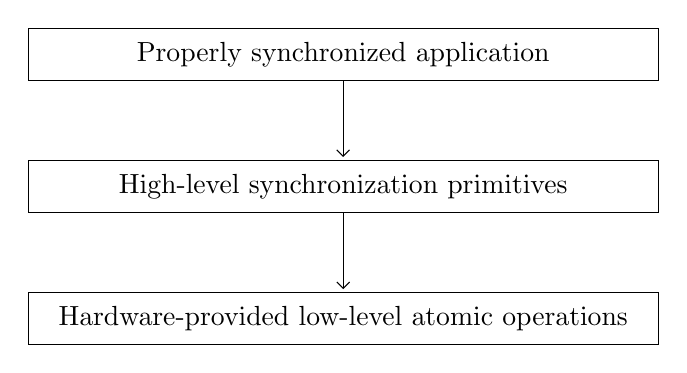
\begin{tikzpicture}[every node/.style={draw, minimum width=8cm, inner sep=0.5em}]
      \node (app) {Properly synchronized application};
      \node [below=of app] (hl) {High-level synchronization primitives};
      \node [below=of hl] (hw) {Hardware-provided low-level atomic operations};
      \draw [->] (app) -- (hl);
      \draw [->] (hl) -- (hw);
    \end{tikzpicture}
  \end{frame}

  \begin{frame}[fragile]
    \frametitle{You Could Use a Lock to Implement Critical Sections}

    Assuming a uniprocessor operating system, you could implement locks as follows:

    \vspace{2em}

    \begin{lstlisting}
void lock() {
  disable_interrupts();
}
void unlock() {
  enable_interrupts();
}   
    \end{lstlisting}

    \vspace{2em}

    This would disable concurrency (assuming it ignores signals and interrupts)

    \hspace{2em} Not going to work on multiprocessors (and OS won't let you change hardware)
  \end{frame}

  \begin{frame}[fragile]
    \frametitle{Let's Try to Implement a Lock in Software}

    \begin{lstlisting}
void init(int *l) {
  *l = 0;
}
void lock(int *l) {
  while (*l == 1);
  *l = 1;
}
void unlock(int *l) {
  *l = 0;
}   
    \end{lstlisting}

    What's the issue with this implementation?

    \vspace{2em}

    \onslide<2->{It's not safe (both threads can be in the critical section)}

    
    \onslide<2->{It's not efficient, it wastes CPU cycles (busy wait)}
  \end{frame}
\end{document}
